\documentclass[a4j,dvipdfmx]{jsarticle}
\usepackage{graphicx}
%\usepackage{multirow}
%\usepackage{color}
%\usepackage{lscape}
%\usepackage{ascmac}
%\usepackage{txfonts}


\usepackage{listings, jlisting}
\renewcommand{\lstlistingname}{リスト}
\lstset{
  language={C},
  basicstyle=\ttfamily\scriptsize,
  commentstyle=\textit,
  classoffset=1,
  keywordstyle=\bfseries,
  frame=tRBl,
  framesep=5pt,
  showstringspaces=true,
  numbers=left,
  stepnumber=1,
  numberstyle=\tiny,
  tabsize=2
}


%% %subsubsubsectionの定義(できるだけ使わない方向で)
%% \makeatletter
%% \newcommand{\subsubsubsection}{\@startsection{paragraph}{4}{\z@}%
%%   {1.0\Cvs \@plus.5\Cdp \@minus.2\Cdp}%
%%   {.1\Cvs \@plus.3\Cdp}%
%%   {\reset@font\sffamily\normalsize}
%% }
\makeatother
\setcounter{secnumdepth}{4}
%ここまでsubsubsubsectionの定義

\begin{document}

\title{計算機科学実験及び演習4\\コンピュータグラフィックス\\課題3}
\author{工学部情報学科3回生 1029255242\\勝見久央}
\date{作成日: \today} % コンパイル時の日付が自動で挿入される
\maketitle
%文字コードはUTF-8推奨.それ以外ではline2のcontentsline~にエラー発生.
%選択範囲コメントアウトは選択中にM-;
%%%%%%%%%%%%%%%%%%%%%%%%%%%%%%%%%%%%%%%%%%%%%%%%%%%%%%%%%%%%%%%%%%%%%%
%ソースコードの貼付け
%% \lstinputlisting[caption=キャプション,label=ラベル,breaklines=true]
%% {./kadai01.sc}
%%次でも可
%% \begin{lstlisting}
%% \end{lstlisting}
\section{概要}
本実験課題では3Dポリゴンデータを透視投影によって投影したPPM画像を生成する
プログラムを課題1のプログラムkadai02.cを拡張させる形でC言語で作成した.
したがって、基本的な仕様は前回のReportForKadai02.pdfに準拠し、
本文では変更点に焦点を当てて言及することとする.

\section{要求仕様}
作成したプログラムが満たす仕様は以下の通りである.
\begin{itemize}
\item ポリゴンデータはVRML形式(拡張子wrl)のファイルで取り込んだ.
\item 光源方向は(x,y,z) = (-1.0, -1.0, 2.0)とした.
\item 光源の明るさは(r,g,b) = (1.0, 1.0, 1.0)とした.
\item 光源モデルは平行光源を採用した.
\item カメラ位置は(x,y,z) = (0.0, 0.0, 0.0)とした.
\item カメラ方向は(x,y,z) = (0.0, 0.0, 1.0)とした.
\item カメラ焦点距離は256.0とした.
\item ポリゴンには拡散反射に加えて鏡面反射を施した.
\item コンスタントシェーディングによりポリゴンを描画した.
\item zバッファによる隠面処理を行った.
\end{itemize}

\section{プログラムの仕様}
\subsection{留意点}
本課題では課題2と同様VRMLファイルの読み込みに与えられた
ルーチンを使用した.なお、使用の方法としてはvrml.cの
main関数は、自分で作成したmain関数の内部に取り込み、
その他の関数についてはそのまま使用した.また、ヘッダファイルも
作成したファイルごとにそのまま参照している.
主な課題2からの変更点については次に示す.
%===========================
\begin{description}
\item[{\bf -ADDED!}]z\_buf[HEIGHT][WIDTH]
\item[{\bf -DEPRECATED}]FILENAME
\item[{\bf -ADDED!}]projected\_ver\_buf[3][2]
\item[{\bf -DEPRICATED!}]void perspective\_pro()
\item[{\bf -MODIFIED!}]void shading(double *a, double *b, double *c, double *n, double *A)
\item[{\bf -ADDED!}]static int strindex(char *s, char *t)
\item[{\bf -ADDED!}]static int getword()
\item[{\bf -ADDED!}]static int read\_material(FILE *fp, Surface *surface, char *b)
\item[{\bf -ADDED!}]static int count\_point(FILE *fp, char *b)
\item[{\bf -ADDED!}]static int read\_point(FILE *fp, Polygon *polygon, char *b)
\item[{\bf -ADDED!}]static int count\_index(FILE *fp, char *b)
\item[{\bf -ADDED!}]static int read\_index(FILE *fp, Polygon *polygon, char *b)
\item[{\bf -ADDED!}]int read\_one\_obj(FILE *fp, Polygon *poly, Surface *surface)
\item[{\bf -MODIFIED!}]main(int argc, char *argv[])
\end{description}
%===========================

\lstinputlisting[caption=vrml.c,label=vrml.c,breaklines=true]
                {./vrml.c}
                
\lstinputlisting[caption=vrml.h,label=vrml.h,breaklines=true]
                {./vrml.h}

\subsection{各種定数}
プログラム内部で使用した重要な定数について以下に挙げておく.
%======================================================================
\subsubsection{ppm}
次の定数はppmファイル生成のための定数である.
kadai01.cと同一のものを使用した.
\begin{itemize}
\item MAGICNUM\\
  ppmファルのヘッダに記述する識別子. P3を使用.
  
\item WIDTH, HEIGHT, WIDTH\_STRING, HEIGHT\_STRING\\
  出力画像の幅、高さ. ともに256とする. STRINGは文字列として使用するためのマクロ.
  以降も同様.
  
\item MAX, MAX\_STRING\\
  RGBの最大値. 255を使用.

\end{itemize}

%======================================================================
\subsubsection{ポリゴンデータ}
課題1のプログラムkadai01.cではポリゴンデータを
関数内部で発生させていたが、課題2以降ではVRMLとしてファイルから取り込むため、
ポリゴンデータを指定する定数は記述していない.

%======================================================================
\subsubsection{環境設定}
次の定数は光源モデルなどの外部環境を特定する定数である.
\begin{itemize}
\item FOCUS\\
  カメラの焦点距離. 256.0と指定.
  
\item light\_dir[3]\\
  光源方向ベクトル.doubel型配列.
  
\item light\_rgb[3]\\
  光源の明るさを正規化したRGB値にして配列に格納したもの.
  double型配列.
  
\end{itemize}

%======================================================================
\subsubsection{その他}
\begin{itemize}
\item image[HEIGHT][WIDTH]\\
  描画した画像の各点の画素値を格納するための領域.
  領域確保のみで初期化は関数内で行う.
  double型の3次元配列.

\item z\_buf[HEIGHT][WIDTH]\\
  zバッファを格納するための領域.全ての頂点分のzバッファを格納する.
  初期化はmain関数内で行う.なお、初期化時の最大値としてはdouble型の最大値
  DBL\_MAXを使用した.
  double型2次元配列.
  
\item projected\_ver\_buf[3][2]\\
  double型2次元配列.
  kadai01.cでのprojected\_verと格納される頂点の意味が異なるため、
  名称を変更をした.
  kadai01.cでは先に全ての頂点をまず透視投影し、その結果を配列
  projected\_verに格納し、その後の操作ではそこから参照を行って使用していたが、
  kadai02.c以降では、空間内の三角形iについてシェーディングを行うという処理をループし、
  処理を行う3頂点ごとに毎回透視投影を施し、その結果をprjected\_ver\_buf
  に格納し、シェーディング時に参照する処理とした.
  これは、ループ処理の構造を設計しやすくするためであり、
  また、透視投影処理の計算の計算量は少ない処理で済むということ、
  頂点座標の数が膨大になると、膨大なメモリ量を確保したにも関わらず、
  一度のループで使用する頂点座標が3点のみであるため、
  直後の処理で使用しない大量の頂点座標のデータのためのメモリ領域を終始確保しなければならず、
  ハード面での無駄が多い、といった点を考慮した結果である.
\end{itemize}

%======================================================================

\subsection{関数外部仕様}
\subsubsection{double func1(double *p, double *q, double y)}
kadai01.cと同一.
double型2次元配列で表された2点p、qの座標とdouble型の値yを引数に取り、
直線pqと直線y=yの交点のx座標をdouble型で返す関数.
ラスタライズの計算を簡素化するために三角形を分割する際に主に用いる.

\subsubsection{int lineOrNot(double *a, double *b, double *c)}
kadai01.cと同一.
double型2次元配列で表された3点a、b、cが一直線上にあるかどうかを判別する関数.
一直線上にある場合はint型1を返し、それ以外のときはint型0を返す.
後述の関数shadingの中で用いる.

\subsubsection{void shading(double *a, double *b, double *c, double *n, double *A)}
内部で変更があるが、外部しようとしてはkadai01.cと同一.
画像平面上に投影されたduble型2次元配列で与えられた3点a、b、cに対してシェーディングを行う関数.

%======================================================================================
\subsection{各関数のアルゴリズムの概要}
\subsubsection{double func1(double *p, double *q, double y)}
kadai01.cと同一.
2点p、qを通る直線の方程式を求めて、直線y=yとの交点を計算する.
なお直線pqがx軸に平行の時はエラーが発生する.

\subsubsection{int lineOrNot(double *a, double *b, double *c)}
kadai01.cと同一.
まず最初に3点a、b、cのx座標が全て同じであるかどうかを判定し、同じであれば一直線上にあると判定する.
同じでなければ、次に点cの座標を直線abの方程式に代入し、等号が成立するかどうかで一直線上に
あるかどうかを判定する。

\subsubsection{void shading(double *a, double *b, double *c, double *n)}
kadai01.cのものを拡張、変更.
主な、変更点としては、shading関数の引数に、シェーディングを行う三角形の法線ベクトルと、
そのうちの一点の座標(ここでは、点Aの座標を用いることとしているが、本来は三角形平面上の一点であれば
  どんなものでも良い.)を加えた.これは、シェーディング時に描画中の三角形内部の点の座標の、
投影平面上のxy座標から元の空間座標を算出し、zバッファと照らしあわせて描画するかどうかを判定するために
使用する.具体的には、投影平面上の点$(x_{p}, y_{p})$の三次元空間内での
座標は、カメラ位置(原点)と投影平面上の点を結ぶ直線と、
xyz空間内の元の三角形ABCを含む平面との交点を求める形で算出でき、元の三角形の法線ベクトルを
$(n_{x}, n_{y}, n_{z})$、点Aでの座標を$(x_{A}, y_{A}, z_{A})$、投影平面のz座標を$z_{p}$
とすると、
\begin{equation}
  \frac{z_{p}(n_{x}x_{A}+n_{y}y_{A}+n_{z}z_{A})}
       {(n_{x}x_{p}) + (n_{y}y_{p}) + (n_{z}z_{p})}
\end{equation}
として、求めることができる.
なお、実際のプログラムでは投影後の点の座標の位置がカメラの中心に周辺に来るように、
平行移動による修正を加えているため、計算時は$x_{p} - \frac{{\rm WIDTH}}{2}$、$y_{p} - \frac{{\rm HEIGHT}}{2}$
を使用した.
これによって算出された値と、zバッファの値を比較し、zバッファよりも大きければ描画せずに次の点の描画
に移り、そうでなければzバッファの値を算出したz座標の値に書き換えてシェーディングを行う.
なお、引数として用いる法線ベクトルと三角形上の点Aの座標はmain関数内で計算し、shading関数内の
再帰呼び出し時は、三角形を分割しても、元の三角形を含む平面とその上の一点の座標は不変であるから、
同じものを使って計算することができる.

\subsubsection{int main(int argc, char *argv[])}
kadai01.cのものを大幅変更、拡張.
作成するPPMファイルの名前をコマンドライン引数として受け取って指定するよう変更を加えた.
前半部分ではコマンドライン引数として受け取ったVRMLファイルを読み込む.
後半部分では三角形ごとにループを行い、その三点のシェーディングを行うため
必要な投影平面上での座標の計算、法線ベクトルの算出(外積から求まる)を行い、
その結果をshading関数に引き渡す.そして、最後に画像の出力を行う.

\section{プログラム本体}
プログラム本体は次のようになった.
\lstinputlisting[caption=kadai02.c,label=kadai02.c,breaklines=true]{./kadai02.c}


\section{実行例}
kadai02.cと同一のディレクトリに次のプログラムを置き、
\lstinputlisting[caption=EvalKadai02.sh,label=EvalKadai02.sh,breaklines=true]{./EvalKadai02.sh}
さらに同一ディレクトリ内のディレクトリsampleの中に対象とするVRMLファイルを置いて、
\begin{lstlisting}
$ sh EvalKadai02.sh
\end{lstlisting}
を実行した.出力画像は最終ページに付与した.

\begin{figure}[hp]
  \begin{center}
    
\includegraphics[clip,scale=0.5]{images/Kadai02ForAv1.eps}
    \caption{av1.wrlの出力結果}
    \label{av1}
  \end{center}
\end{figure}

\begin{figure}[hp]
  \begin{center}
    
\includegraphics[clip,scale=0.5]{images/Kadai02ForAv2.eps}
    \caption{av2.wrlの出力結果}
    \label{av2}
  \end{center}
\end{figure}

\begin{figure}[hp]
  \begin{center}
    
\includegraphics[clip,scale=0.5]{images/Kadai02ForAv3.eps}
    \caption{av3.wrlの出力結果}
    \label{av3}
  \end{center}
\end{figure}

\begin{figure}[hp]
  \begin{center}
    
\includegraphics[clip,scale=0.5]{images/Kadai02ForAv4.eps}
    \caption{av4.wrlの出力結果}
    \label{av4}
  \end{center}
\end{figure}

\begin{figure}[hp]
  \begin{center}
    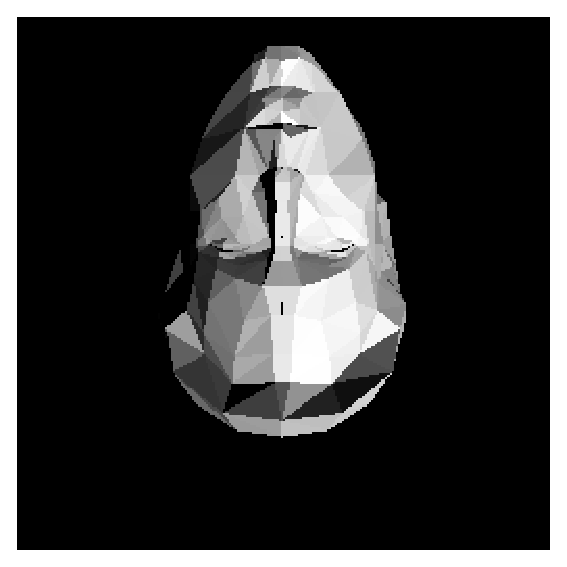
\includegraphics[clip,scale=0.5]{images/Kadai02ForHead.eps}
    \caption{head.wrlの出力結果}
    \label{head}
  \end{center}
\end{figure}

\begin{figure}[hp]
  \begin{center}
    
\includegraphics[clip,scale=0.5]{images/Kadai02ForIiyama1997.eps}
    \caption{iiyama1997.wrlの出力結果}
    \label{1997}
  \end{center}
\end{figure}

\section{工夫点、問題点、感想}
前半部分でも述べたように、自分としてはできるだけ計算の処理や、使用するメモリ量を節約し、
無駄なデータを長時間大量に保持する事のないようにプログラムを書いたつもりである.
C言語はJava等と比べて、プログラマがハード面の挙動にも気を使ってプログラムを書く必要があるが、
レンダリングなどの大量の計算処理を行う必要のあるプログラムでは、
普段の実験で書くようなプログラムよりも一層、無駄のないプログラムを書く必要性があるのだと感じた.
実際、最初の段階でうまく設計をしなかったために途中で膨大な場合分けが発生してしまい、
気をつけて書いたつもりでも、emacs上で動かすシェルでは動作が重すぎて、一つのVRMLを表示させるのに
数分かかってしまったこともあった.また、リアルタイムでレンダリング処理を行うゲーム機などでは
そういった処理を一瞬で行っているという凄さに改めて気付かされ、そういった部分にも興味が湧いた.


\section{APPENDIX}
ベースとしたkadai01.cのプログラムを付加しておく.
\lstinputlisting[caption=kadai01.c,label=kadai01.c,breaklines=true]{./kadai01.c}

\end{document}
